\chapter{Filtros Digitales}

En este capítulo veremos como es el diseño de un filtro digital a partir de uno analógico, y para ello utilizaremos lo que se conoce como \textbf{Transformación Bilineal}. Esta transformación mapea el plano complejo del dominio de frecuencia analógico al dominio de frecuencia digital utilizando una relación no lineal.

Es importante tener en cuenta que la transformación bilineal introduce distorsiones en la respuesta en frecuencia del filtro analógico original al convertirlo en un filtro digital, como se muestra en la Figura \ref{fig:distorsion_frecuencia_angular}. Estas distorsiones son inevitables debido a la naturaleza no lineal de la transformación. Sin embargo, en muchos casos, estas distorsiones son aceptables y se pueden compensar mediante técnicas de diseño adicionales. Una de estas técnicas es el \textbf{Pre-Warping}.

\begin{figure}[H]
  \centering
  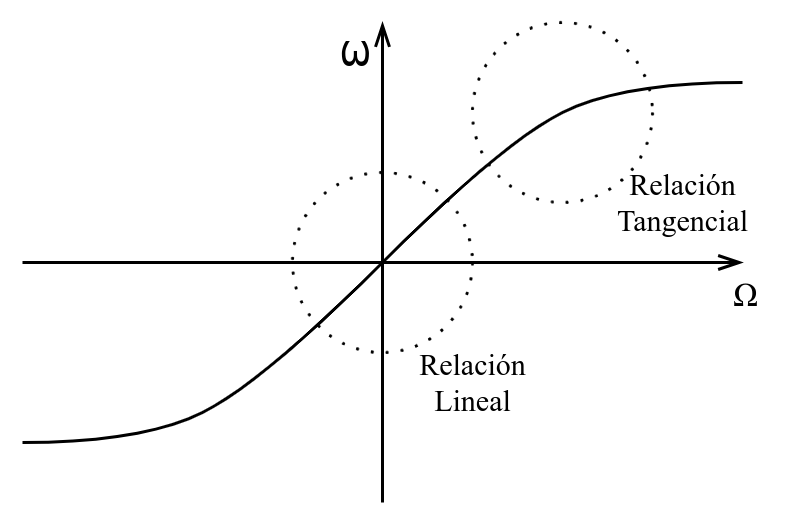
\includegraphics[width=300pt]{images/diagramas-distorsion-frecuencia-angular.png}
  \caption{Distorsion de frecuencia introducida por la Transformación Bilineal}
  \label{fig:distorsion_frecuencia_angular}
\end{figure}

El pre-warping es un ajuste realizado a la frecuencia de corte del filtro analógico antes de aplicar la transformación. Se hace con el fin de compensar la distorsión introducida por la transformación bilineal en las frecuencias más altas, esto es debido a la no linealidad de la función tangente utilizada en la transformación.

El pre-warping ajusta la frecuencia de corte del filtro analógico antes de aplicar la transformación bilineal para compensar esta distorsión. Se utiliza una función que aproxima la inversa de la función tangente hiperbólica para ajustar la frecuencia de corte en el dominio analógico.

Para más información acerca de la Transformación Bilineal se pueden consultar en las siguientes bibliografías: \cite{proakis1996digital}, \cite{oppenheim1989discrete} y \cite{oppenheim1999digital}.

\section{Diseño}
Primero, se diseña el filtro analógico deseado utilizando un método de diseño como el filtro Butterworth, Chebyshev o el filtro elíptico. En este caso usaremos el filtro Butterworth. Este se caracteriza por tener una respuesta en frecuencia lo más plana y suave posible en la banda de paso, lo que significa que atenúa las frecuencias no deseadas de manera gradual y sin oscilaciones abruptas.

El filtro de Butterworth más típico es el filtro pasa bajo de primer orden, el cual puede ser modificado a un filtro pasa alto o añadir en serie otros formando un filtro pasa banda o elimina banda y filtros de mayores órdenes; esta composición de filtros es la que se busca, como describre la Figura \ref{fig:diagrama_filtro_pasa_banda}. Este filtro será el utilizado para demostrar el proceso de diseño.

\begin{figure}[H]
  \centering
  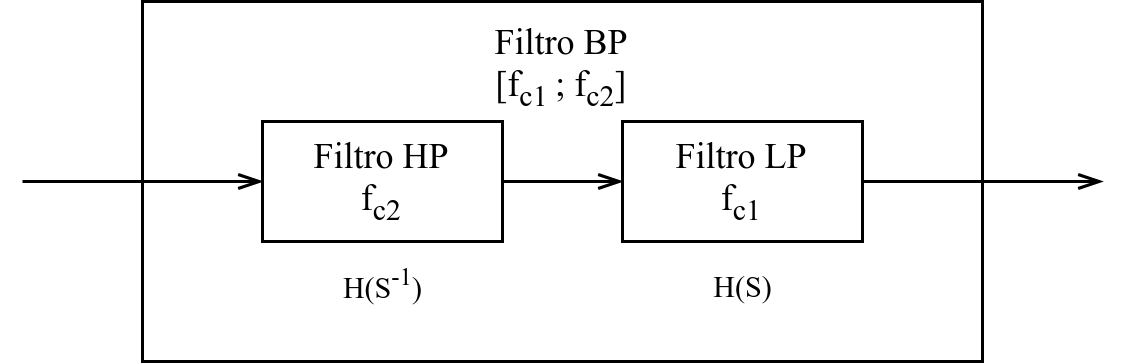
\includegraphics[width=400pt]{images/diagramas-bloques-pasa-banda.png}
  \caption{Filtro pasa-banda a partir de filtros pasa-alto y pasa-alto de Butterworth}
  \label{fig:diagrama_filtro_pasa_banda}
\end{figure}

\begin{figure}[H]
  \centering
  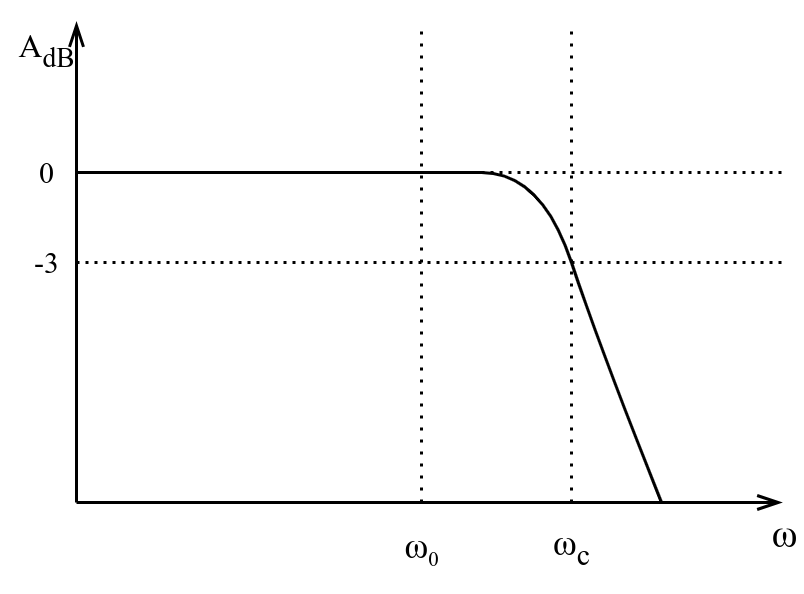
\includegraphics[width=300pt]{images/diagramas-bode-pasa-bajo.png}
  \caption{Respuesta en frecuencia de un filtro pasa-bajos}
  \label{fig:diagrama_bode_pasa_bajos}
\end{figure}

El siguiente paso elegir las frecuencias con las que va a operar el filtro. Para ello tomamos la frecuencia baja de de los digitos 1, 2 y 3 (ver Cuaddro \ref{tab:combinacion_tonos}), que resulta ser la frecuencia más baja del espectro de este dominio. Esta elección no es arbitraria, ya que al ser la frecuencia más baja, podemos usar un filtro pasa-bajos para filtrar el resto de señales que son mayores, como describe la Figura \ref{fig:diagrama_bode_pasa_bajos}. Para este caso, la frecuencia de corte será 60 [Hz] por encima de la frecuencia entral, es decir, $f_c=f_0+60\textrm{[Hz]}=757\ \textrm{[Hz]}$. Recordemos que para pasar frecuencia angular analógica debemos realizar el pre-warping. Entonces la frecuencia angular de corte analógica está dada por la Ecuación \ref{eq:frecuencia_angular_analogica}, donde \gls{fs} es igual a 44 [kHz].

\begin{equation}
  \omega_{c} = 2 f_s \tan \frac{\pi f_c}{f_s} = 4761,01\ \mathrm{\left[\frac{rad}{s}\right]}
  \label{eq:frecuencia_angular_analogica}
\end{equation}


Lo siguiente será encontrar los coeficientes del filtro pasa-bajos Butterworth, y para eso utilizaremos los polinomios normalizados de Butterworth. Los coeficientes de estos polinomios son valores tabulados para filtro de frecuencia de 1 radian por segundo. Para un filtro de primer orden la función transferencia está dada por la Ecuación \ref{eq:fn_transf_pb_n1}. Sin embargo esta función está normalizada, es decir que es un filtro con frecuencia de corte de 1 rad/s. Para poder obtener la función transferencia correctas debemos desnormalizarla, y esto se logra reemplazando $s$ por $\frac{s}{\omega_c}$. En la Ecuación \ref{eq:fn_transf_pb_n1_desnormalizada} obtenemos la función transferencia correcta para una $\omega_c = 4761,01\ \mathrm{\left[\frac{rad}{s}\right]}$.

\begin{equation}
  H(s) = \frac{1}{s+1}
  \label{eq:fn_transf_pb_n1}
\end{equation}

\begin{equation}
  H(s) = \frac{1}{\frac{s}{\omega_c}+1} = \frac{\omega_c}{s + \omega_c}
  \label{eq:fn_transf_pb_n1_desnormalizada}
\end{equation}

Con esto sería suficiente si el objetivo fuera diseñar un filtro pasa-bajos, sin embargo se busca es diseñar un filtro pasa-banda, cuya respuesta en frecuencia sea como en la Figura \ref{fig:diagrama_bode_pasa_banda}. Como se puede ver, la parte derecha del gráfico es referente al filtro pasa-bajos, la de la izquierda es del filtro pasa-altos, el cual procedemos a diseñar.

\begin{figure}[ht!]
  \centering
  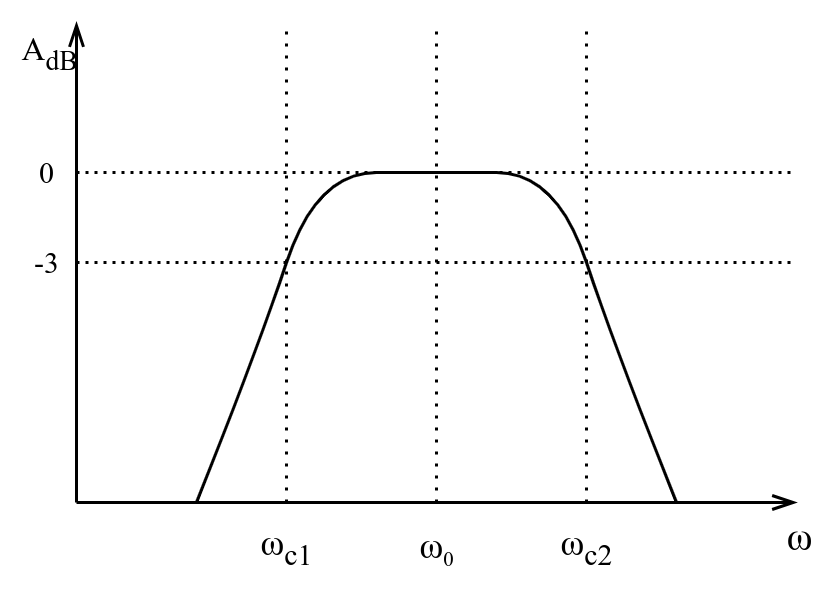
\includegraphics[width=300pt]{images/diagramas-bode-pasa-banda.png}
  \caption{Respuesta en frecuencia de un filtro pasa-banda}
  \label{fig:diagrama_bode_pasa_banda}
\end{figure}

Al igual que el filtro pasa-bajos, necesitamos establecer la frecuencia de corte analógica teniendo en cuenta el pre-warping. Como la frecuencia de corte superior es 60 [Hz] por encima de la frecuencia central, análogamente la frecuencia de corte inferior será 60 [Hz] por debajo de la frecuencia central (637 [Hz]). A estas frecuencias angulares de corte analógicas las llamaremos $\omega_{c1}$ (inferior) y $\omega_{c2}$ (superior). En la Ecuación \ref{eq:omega_corte_analogica_inferior} vemos como se obtiene $\omega_{c1}$, luego en la Ecuación \ref{eq:fn_transf_pa_n1} vemos la forma de la función transferencia de un filtro pasa-alto normalizado\footnote{En el caso de los filtros pasa-altos, no existen una función transferencia determinada, sin embargo podemos calcularlo reemplazando $s$ por $\frac{1}{s}$ en la función transferencia del filtro pasa-bajos.}. Para encontrar la función transferencia desnormalizada el procedimiento es similar al del filtro pasa-bajos solo que ahora la frecuencia de corte angular será diferente, como se muestra en la Ecuación \ref{eq:fn_transf_pa_n1_desnormalizada}.

\begin{equation}
  \omega_{c1} = 2 f_s \tan \frac{\pi f_{c1}}{f_s} = 4000,15\ \mathrm{\left[\frac{rad}{s}\right]}
  \label{eq:omega_corte_analogica_inferior}
\end{equation}

\begin{equation}
  H(s) = \frac{1}{\frac{1}{s}+1} = \frac{s}{s+1}
  \label{eq:fn_transf_pa_n1}
\end{equation}

\begin{equation}
  H(s) = \frac{\frac{s}{\omega_{c1}}}{\frac{s}{\omega_{c1}}+1} = \frac{s}{s + \omega_{c1}}
  \label{eq:fn_transf_pa_n1_desnormalizada}
\end{equation}

Ahora que tenemos $H(s)$ para cada filtro podemos calcular la función transferencia del filtro pasa-banda que resulta del producto de ambas $H(s)$, como se muestra en la Ecuación \ref{eq:fn_transf_pb} Al trabajarlo algebraicamente llegamos a la $H(s)$ del filtro pasa-banda.

\begin{align}
  H(s) & = H_{HP}(s) H_{LP}(s)                                                                 \\
  H(s) & = \frac{s}{s+\omega_{c1}}\frac{\omega_{c2}}{s+\omega_{c2}}                            \\
  H(s) & = \frac{\omega_{c2}\ s}{s^2  + (\omega_{c1} + \omega_{c2})s + \omega_{c1}\omega_{c2}} \\
  H(s) & = \frac{4761,01\ s}{s^2 + 8766,16\ s + 19,07\times 10^6}
\end{align}

\begin{equation}
  H(s) = \frac{s}{s+\omega_{c1}}\frac{\omega_{c2}}{s+\omega_{c2}}
  \label{eq:fn_transf_pb}
\end{equation}


\section{Conversión a digital}

\section{Análisis}

\section{Conclusiones}